\subsection{Desarrollo del Método DCF}

\textcolor{principal}{An\'alisis Hist\'orico de los Ingresos y Flujos operativos del Negocio.}\\

El perito valuador llev\'o a cabo el an\'alisis financiero de los ingresos (\textit{Revenues}) y de la utilidad operativa del negocio (Ebit) del periodo de \EFdeHasta, con el objetivo de usar de base dicho an\'alisis para proyectar correctamente los flujos de operaci\'on de la sociedad en la aplicaci\'on del modelo DCF como m\'etodo principal para determinar el valor razonable de la firma.

\begin{figure}[H]
\centering
\includegraphics[width=14cm]{../0.imagenes/dcf_1}
\end{figure}

\begin{figure}[H]
\centering
\includegraphics[width=8cm]{../0.imagenes/dcf_2}
\end{figure}


\textcolor{principal}{\textbf{PROYECCI\'ON FINANCIERA.} Proyecci\'on de Ingresos y del Flujo de Operaci\'on del Negocio.} El perito valuador llev\'o a cabo la proyecci\'on del EBIT de la sociedad del periodo \periodoProyeccion. Como premisas de la proyecci\'on se utilizaron los siguientes indicadores (\textit{ceteris paribus}): i) \gls{cagr} \periodoProyeccion: \proyCagr\%, ii) Margen Operativo (\textit{Ebit margin}): \proyEbitMargin\%.

\begin{figure}[H]
\centering
\includegraphics[width=15cm]{../0.imagenes/dcf_proy}
\end{figure}

\textbf{\textcolor{principal}{Estimaci\'on del Flujo de Efectivo Libre a la Firma (\gls{fcff}).}} El valuador llev\'o a cabo la estimaci\'on del Flujo de Caja Libre a la firma
%, conforme a la metodolog\'ia conocida como ``Ebit sintetizado'', la cual estima dos premisas: i) El flujo de operaci\'on neto o \gls{nopat} (INFLOWS) y  ii) Los cambios al capital invertido (OUTFLOWS)
. Dicha estimaci\'on representa la capacidad de la empresa de generar flujo de efectivo con sus activos operativos. La productividad de un activo se mide en funci\'on de la capacidad de generar rentabilidad para sus accionistas y fondeadores.\\

Se utilizaron las siguientes premisas (\textit{ceteris paribus}): i) Tasa fiscal efectiva (\gls{etr}): \tasaFiscal\%, ii) Tasa de Reinversi\'on (\textit{Reinvestment Rate}): \reinvestmentRate\%. Los resultados de la proyecci\'on se detallan a cotinuaci\'on:

\begin{figure}[H]
\centering
\includegraphics[width=15cm]{../0.imagenes/FCFF}
\end{figure}



\textcolor{principal}{OBTENCI\'ON DEL INDICADOR DE VALOR DE LA FIRMA Y DEL NEGOCIO MEDIANTE EL M\'ETODO DCF.} Se analiz\'o el modelo explicado, el cual cuenta con amplia aceptaci\'on en la valuaci\'on de negocios a nivel mundial.  Sus resultados se exhiben a continuaci\'on:

\begin{figure}[H]
\centering
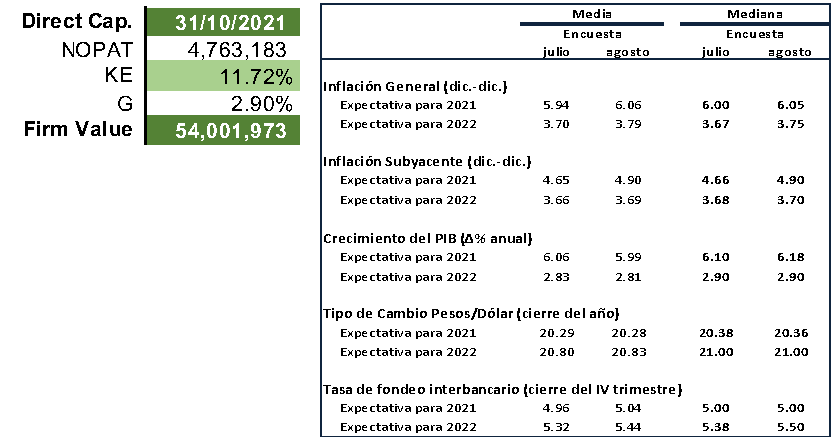
\includegraphics[width=14cm]{../0.imagenes/valor_dcf}\\
\textcolor{principal}{\textbf{\textbullet Valor razonable del negocio en marcha: \$\valorDCF{} MXN}}
\end{figure}
